% English–Dhivehi MT paper — humanized (bachelor-student voice) revision of main.tex
% compile with XeLaTeX: tectonic paper/main_humanized.tex
\documentclass[10pt,twocolumn]{article}

\usepackage[margin=2.2cm,columnsep=0.7cm]{geometry}
\usepackage{booktabs}
\usepackage{graphicx}
\usepackage{amsmath}
\usepackage{url}
\usepackage[numbers,sort&compress]{natbib}
\usepackage{pgfplots}
\pgfplotsset{compat=1.18}
\usepackage{fontspec}
\usepackage[hidelinks]{hyperref}
\usepackage{bidi} % must be loaded last

% Script=Thaana is load-bearing: without it the shaper treats runs as
% neutral/LTR and every fili attaches to the wrong consonant
\newfontfamily\thaanafont[Path=fonts/, Extension=.ttf, Script=Thaana]{Faruma}
\newcommand{\dv}[1]{{\thaanafont\RL{#1}}}
% paragraph-level RTL for table cells: \RL boxes can't wrap, so multi-line
% Thaana in p{} columns needs \setRTL active while the paragraph is built
\newcommand{\dvcell}[1]{{\thaanafont\setRTL #1\par}}

% ---- pending comparison numbers: filled after eval runs ----
\newcommand{\resSevenChrf}{17.83$^\dagger$}
\newcommand{\resSevenBleu}{8.78}
\newcommand{\resSevenRt}{80.3\%}
\newcommand{\resTGChrf}{33.18}
\newcommand{\resTGBleu}{40.83}
\newcommand{\resTGRt}{96.3\%}
\newcommand{\resGFourChrf}{23.22}
\newcommand{\resGFourBleu}{25.52}
\newcommand{\resGFourRt}{48.3\%}
\newcommand{\resQwenChrf}{3.89}
\newcommand{\resQwenBleu}{1.35}
\newcommand{\resQwenRt}{92.3\%}

\title{\Large\bf Pretraining Coverage Beats Scale:\\
A Strong English--Dhivehi Model and Benchmark}
\author{streetsolider\\
\small Independent researcher\\
\small \url{https://github.com/streetsolider}}
\date{August 2026}

\begin{document}
\maketitle

\begin{abstract}
Dhivehi is the national language of the Maldives. It is spoken by nearly
half a million people and is written in Thaana, a right-to-left script
that no other language uses. Despite this, none of the major open translation models
support it: NLLB-200 does not include it, FLORES-200 has no Dhivehi data,
and Google's recent TranslateGemma models do not list it among their
benchmarked languages either. In this paper we describe how we trained a
usable English$\to$Dhivehi translation model with modest compute. We
started from MADLAD-400 3B-MT, a T5-style encoder--decoder pretrained for
translation across more than 450 languages, whose 256k-token vocabulary
and pretraining corpus both cover Thaana; we confirmed this fit by
measuring how efficiently different models' tokenizers encode Thaana
text. We then fine-tuned it with LoRA on about 93{,}000 cleaned
news-domain sentence pairs, roughly 10 GPU-hours of training. On a
frozen test set of 1{,}500 sentence pairs, the chrF++ score improved from
42.6 (the model as downloaded) to \textbf{61.8}, and every output passed an
automatic script-validity check that round-trips the text through the Segha
keymap, a one-to-one mapping between Thaana characters and ASCII. We also
compared against larger open models used out of the box (a quantized
MADLAD 7B and the instruction-tuned LLMs TranslateGemma 12B, Gemma~4 12B
and Qwen3 14B) and against earlier community fine-tunes for this
direction; all of them scored below the fine-tuned 3B model. The
strongest earlier system, an mT5-large trained on synthetic targets,
trails it by 6 chrF++ on the same benchmark. The evaluation set
construction steps, training code, and the LoRA adapter are released.
\end{abstract}

\section{Introduction}

Machine translation now covers hundreds of languages, but the coverage is
uneven, and Dhivehi (ISO 639-1 \texttt{dv}) is a clear example of a
language that has been left out. It is an Indo-Aryan language, the official
language of the Maldives, and it is written in Thaana, a right-to-left
script used by no other language. Because the speaker population is small,
most large multilingual projects simply skip it. NLLB-200 \citep{nllb}
covers 202 languages, and Dhivehi is not one of them. Its companion
benchmark FLORES-200 therefore has no Dhivehi portion, and neither did the
earlier FLORES-101 \citep{flores101}. TranslateGemma
\citep{translategemma}, Google's 2026 family of open translation models,
reports results for 55 languages on WMT24++ \citep{wmt24pp}, and Dhivehi
is again absent. (Google Translate does support Dhivehi, but it is a
closed commercial service, not something a researcher can inspect, run
locally, or build on.) As far as we could find, there is no public
benchmark for Dhivehi and no open translation model whose pretraining
actually covered the language; what does exist publicly for
English$\to$Dhivehi is a handful of community fine-tunes
\citep{flant5endv,neobeendv}, and we evaluate all of them on our
benchmark in \S\ref{sec:results}.

The question this paper tries to answer is a practical one: how far can
careful base-model selection and parameter-efficient fine-tuning close
that gap? The main contributions are:

\begin{enumerate}
  \item \textbf{A simple way to pick a base model for an unusual script.}
  Before doing any training, we measured subword fertility (the average
  number of tokens a tokenizer needs per word) on real Thaana text for
  several open models (\S\ref{sec:model}). The differences were large:
  about a $6\times$ spread between MADLAD-400's tokenizer and the
  tokenizers of recent general-purpose LLMs.
  \item \textbf{A cleaned training corpus and a frozen benchmark} for
  English$\to$Dhivehi, built only from permissively licensed public data
  (\S\ref{sec:data}): 93{,}258 training pairs, a 1{,}000-pair development
  set, and a frozen, topic-stratified 1{,}500-pair test set.
  \item \textbf{An automatic script-validity check.} Every output is
  round-tripped through the Segha keymap \citep{divtransliteration}, a
  one-to-one mapping between Thaana codepoints and ASCII characters. If an
  output contains anything that is not valid Thaana (plus allowed
  punctuation and digits), the round trip changes the string and the error
  is caught automatically (\S\ref{sec:keymap}).
  \item \textbf{Strong results from a well-matched base model.} LoRA
  fine-tuning of MADLAD-400 3B-MT for about 10 GPU-hours improved chrF++
  by +19.2 points over the base model, and the result beats much larger
  out-of-the-box open models, including ones specialized for translation
  (\S\ref{sec:results}).
  \item \textbf{A reproducibility note} about a silent bug when loading
  MADLAD checkpoints under \texttt{transformers} 5.x. The bug ties the
  wrong weight matrices together and quietly turns the model's output into
  garbage (Appendix~\ref{app:bug}).
\end{enumerate}

\section{Background}

\subsection{Dhivehi and Thaana}

Dhivehi is spoken by nearly half a million people
\citep{ethnologue28,census2022}, counting the resident population of the
Maldives and the Mahl-speaking community on the Indian island of Minicoy.
Thaana is written right-to-left. Every consonant letter carries an
obligatory vowel diacritic (called \emph{fili}), so well-formed text
alternates between base characters (U+0780--U+07A5) and combining marks
(U+07A6--U+07B0). Dhivehi morphology leans agglutinative, with long
inflected verb forms; the news register in particular uses distinctive
sentence-final perfective verb forms (for example, verbs ending in
\dv{ކޮށްފި} in headlines). Standard Dhivehi text uses Arabic-script
punctuation (\dv{،} \dv{؛} \dv{؟}) rather than the ASCII equivalents.

\subsection{The Segha keymap as a validity check}
\label{sec:keymap}

The Segha keymap \citep{divtransliteration} maps each Thaana codepoint to
a single printable ASCII character and back. It was originally built for
keyboard input and transliteration, but the fact that the mapping is
one-to-one gives it a second use. For any string $s$ that consists only of
valid Thaana characters, common punctuation, digits, and whitespace,
$\mathrm{key2thaana}(\mathrm{thaana2key}(s)) = s$. If the string contains
anything else (mojibake, a stray Latin fragment, an Arabic-script
character outside the allowed set, or an invalid codepoint), the round
trip does not reproduce the input. We report the \emph{round-trip pass
rate}, the fraction of model outputs that survive this round trip
unchanged, as a script-validity metric alongside the translation quality
metrics. It is cheap and deterministic, and it catches a failure mode
(mixing scripts) that chrF++ only penalizes weakly. The same module also
supplies the punctuation normalization used during data preparation
(mapping ASCII \texttt{,;?} to their Arabic counterparts).

\section{Related work}

MADLAD-400 \citep{madlad400} released a 3-trillion-token audited corpus
covering 419 languages, along with T5-based \citep{t5} translation models
trained on more than 450 languages. This matters here because they are, to
our knowledge, the only strong open checkpoints whose training data
genuinely includes Dhivehi (about 3.5M clean sentences). NLLB-200
\citep{nllb} is the usual reference open system for low-resource
translation, but it omits Dhivehi entirely. GATITOS \citep{gatitos} and
SMOL \citep{smol} provide small professionally translated English--Dhivehi
wordlists and sentences. On the data side, alakxender
\citep{dhivehienglishtranslations} has published aligned news-domain
sentence pairs; their own MT models mostly target the dv$\to$en
direction, with en$\to$dv, the direction needed to make content
available \emph{in} Dhivehi, covered only by a 250M multi-task
Flan-T5 \citep{flant5endv}. Neobe \citep{neobeendv} released dedicated
en$\to$dv fine-tunes (mT5-large, ByT5-large, and a Qwen3-4B LoRA),
trained on machine-translated (synthetic-target) news and Wikipedia
text. NLLB-based Dhivehi fine-tunes also exist, but they target
romanized Dhivehi (\texttt{div\_Latn}) rather than Thaana. We evaluate
the Thaana-native systems on our benchmark in \S\ref{sec:results}.
Finally, LoRA \citep{lora}
and 4-bit NF4 quantization \citep{qlora} keep the fine-tuning and the
7B-scale comparison runs affordable.

\section{Choosing a base model with tokenizer fertility}
\label{sec:model}

A model is unlikely to translate well into a script that its tokenizer can
only represent as individual bytes. To check this before training
anything, we measured fertility (subword tokens per whitespace-separated
word) on the 13{,}763 Dhivehi words in the frozen test set
(Table~\ref{tab:fertility}).

\begin{table}[t]
\centering\small
\begin{tabular}{lrr}
\toprule
Tokenizer & tok/word & rel.\ to MADLAD \\
\midrule
NLLB-200          & 2.78 & $0.96\times$ \\
MADLAD-400        & \textbf{2.89} & $1.00\times$ \\
Gemma-3           & 5.93 & $2.05\times$ \\
Qwen3             & 16.05 & $5.55\times$ \\
BLOOM             & 16.26 & $5.63\times$ \\
OLMo-2            & 17.15 & $5.93\times$ \\
\bottomrule
\end{tabular}
\caption{Subword fertility on the Thaana side of the test set. MADLAD's
256k SentencePiece vocabulary contains whole Thaana words, while most
recent LLM tokenizers fall back to bytes. NLLB's tokenizer handles Thaana
well, but the model itself was never trained on Dhivehi; tokenizer
coverage alone is not enough.}
\label{tab:fertility}
\end{table}

MADLAD-400 and NLLB-200 tokenize Thaana compactly, while the
general-purpose LLMs need 5--6$\times$ more tokens for the same text. That
overhead hurts twice: the training targets become much longer (which
spreads the learning signal thinner), and inference gets proportionally
more expensive. Tokenizer coverage then combines with training-data
coverage: MADLAD is the only model in the table that actually saw Dhivehi
during pretraining. This pointed clearly at \texttt{madlad400-3b-mt}, a
3B-parameter T5-style encoder--decoder with a 256k SentencePiece
vocabulary, trained for translation across more than 450 languages, which
selects its target language with a task prefix (\texttt{<2dv> \{English
text\}}). The encoder--decoder architecture also suits the task: the
whole English sentence is encoded bidirectionally before any Thaana is
generated, unlike in a decoder-only LLM. We picked the 3B size rather
than 7B or 10B because it is the largest that still allows unquantized
bf16 LoRA training within 16\,GB.

\section{Data}
\label{sec:data}

\textbf{Sources.} For this first round we used only the cleanest
permissively licensed public data: (i) \texttt{dhivehi-english-translations}
\citep{dhivehienglishtranslations}, 82{,}583 news-domain sentence pairs
with topic labels (MIT license); and (ii) the GATITOS en--dv data
\citep{gatitos,smol}, 3{,}973 professionally translated words and short
phrases (CC-BY-4.0), which we upsampled $3\times$ so the model gets
repeated exposure to reliable terminology. We deliberately left out the
larger but noisier options (a 484k mixed-granularity crawl, and synthetic
distillation sets); the synthetic sets in particular could contaminate any
test set built from public news text.

\textbf{Cleaning.} Dhivehi text is normalized to Unicode NFC, and ASCII
punctuation is mapped to its Arabic equivalents using the keymap module's
rules. Pairs are dropped unless the target side is at least 70\% Thaana
characters, and pairs with a source/target length ratio outside
$[0.25, 4.0]$ are filtered out.

\textbf{Splits.} From the source dataset's held-out test partition we froze
two sets: \emph{devtest} (1{,}500 pairs, topic-stratified, used only for
final reporting) and \emph{dev} (1{,}000 pairs, used for checkpoint
selection). The training data was deduplicated against both splits on both
language sides, leaving \textbf{93{,}258} training pairs.

\section{Fine-tuning setup}
\label{sec:setup}

We trained LoRA \citep{lora} adapters ($r{=}32$, $\alpha{=}64$, dropout
0.05) on all attention projections and feed-forward matrices of the
encoder, decoder, and cross-attention (94.4M trainable parameters, or
3.1\% of the model) in bf16, with gradient checkpointing and the 8-bit
AdamW optimizer. The effective batch size is 64 (8 per device $\times$ 8
gradient-accumulation steps), the learning rate is $10^{-4}$ with cosine
decay and 200 warmup steps, and training ran for 3 epochs (4{,}374 steps),
about 10.3 hours end-to-end on our single 16\,GB GPU. Every 400 steps we
decoded a fixed 500-sample subset of the dev set greedily and kept the
checkpoint with the best dev chrF++ (61.45, reached at step 4{,}000;
Figure~\ref{fig:curve}). Full hyperparameters are listed in
Appendix~\ref{app:hparams}.

\begin{figure}[t]
\centering
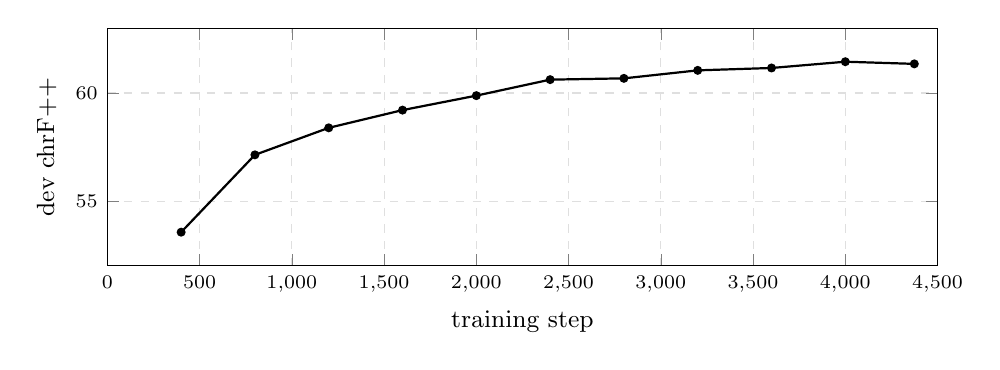
\begin{tikzpicture}
\begin{axis}[
  width=\linewidth, height=4.6cm,
  xlabel={training step}, ylabel={dev chrF++},
  xmin=0, xmax=4500, ymin=52, ymax=63,
  grid=major, grid style={dashed,gray!25},
  tick label style={font=\scriptsize},
  label style={font=\small},
  mark size=1.2pt,
]
\addplot[thick,mark=*] coordinates {
(400,53.56)(800,57.14)(1200,58.39)(1600,59.21)(2000,59.88)
(2400,60.62)(2800,60.68)(3200,61.05)(3600,61.16)(4000,61.45)(4374,61.35)
};
\end{axis}
\end{tikzpicture}
\caption{Development chrF++ (greedy decoding, 500-sample subset) during
fine-tuning. The best checkpoint (step 4{,}000) is used for all reported
results.}
\label{fig:curve}
\end{figure}

\section{Evaluation protocol}

All systems are scored on the frozen devtest set with sacreBLEU
\citep{sacrebleu}. The headline metric is \textbf{chrF++} \citep{chrfpp}
(with word order 2), a character-level F-score that is better suited to a
morphologically rich language like Dhivehi than word-level BLEU. As a
secondary metric we report character-level BLEU (word-level BLEU is
unreliable here because Thaana words carry so much inflection), plus the
keymap round-trip pass rate from \S\ref{sec:keymap}. The MADLAD-family
systems decode with beam size 4. The instruction-tuned LLMs are evaluated
zero-shot with a fixed prompt (Appendix~\ref{app:prompt}) at temperature
0. Because running them is slow, they are scored on a fixed random
400-pair subset of devtest (seed 13); the fine-tuned model and the 3B
baseline are re-scored on that identical subset so the comparison is
like-for-like.

\section{Results}
\label{sec:results}

\begin{table}[t]
\centering\small
\begin{tabular}{lrrr}
\toprule
System & chrF++ & BLEU$_c$ & RT \\
\midrule
\multicolumn{4}{l}{\emph{Full devtest (1{,}500), beam 4}}\\
madlad400-3b-mt (base)       & 42.59 & 48.36 & 94.6\% \\
madlad400-7b-mt-bt (NF4)     & \resSevenChrf{} & \resSevenBleu{} & \resSevenRt{} \\
Flan-T5 en2dv 250M \citep{flant5endv} & 24.90 & 11.09 & 53.8\% \\
Neobe ByT5-large 1.2B \citep{neobeendv} & 49.61 & 60.07 & 100\% \\
Neobe mT5-large 1.2B \citep{neobeendv} & 55.75 & 67.15 & 100\% \\
\textbf{3B + LoRA (ours)}    & \textbf{61.82} & \textbf{72.21} & \textbf{100\%} \\
\midrule
\multicolumn{4}{l}{\emph{400-pair subset, zero-shot instruction LLMs}}\\
TranslateGemma 12B (q4)      & \resTGChrf{} & \resTGBleu{} & \resTGRt{} \\
Gemma 4 12B (qat)            & \resGFourChrf{} & \resGFourBleu{} & \resGFourRt{} \\
Qwen3 14B (q4)               & \resQwenChrf{} & \resQwenBleu{} & \resQwenRt{} \\
madlad400-3b-mt (base)       & 42.19 & 47.49 & 93.3\% \\
\textbf{3B + LoRA (ours)}    & \textbf{62.77} & \textbf{73.16} & \textbf{100\%} \\
\midrule
NLLB-200 & \multicolumn{3}{c}{\emph{no Dhivehi support}} \\
\bottomrule
\end{tabular}
\caption{English$\to$Dhivehi results. BLEU$_c$ = character-level BLEU; RT =
Segha keymap round-trip pass rate. Quantization is noted in parentheses.
$^\dagger$Falls into repetition loops on about half of the inputs under
NF4; \S\ref{sec:results} breaks this down.}
\label{tab:main}
\end{table}

Fine-tuning improves the 3B model by \textbf{+19.2 chrF++} (42.6 $\to$
61.8) and \textbf{+23.9} character BLEU, and closes the script-validity
gap (94.6\% $\to$ 100\% round-trip). The base model occasionally emits
stray Latin characters or malformed sequences; on this test set, the
fine-tuned model never does (Table~\ref{tab:main}).

The instruction-LLM rows show two different ways a model can fail.
Gemma~4 produces non-Thaana content in about half of its outputs (48.3\%
round-trip). Qwen3 is almost the opposite: its round-trip rate is high
(92.3\%) but its chrF++ is close to zero, because it tends to fall into
repetition loops of valid Thaana words, and sometimes answers in the wrong
script altogether (Sinhala or Arabic). In other words, script validity is
necessary but not sufficient: the round-trip metric is meant to
complement the quality metrics, not replace them. TranslateGemma, the
strongest of the LLM rows, produces mostly valid Thaana but still scores
below the \emph{untuned} MADLAD 3B baseline, which is consistent with
Dhivehi being outside its supported language set.

The quantized 7B row needs some unpacking. Under NF4,
\texttt{madlad400-7b-mt-bt} falls into repetition loops on roughly half
the test set (32\% of its outputs contain no Thaana at all, and its
average output is four times as long as the reference), which collapses
its corpus-level score. On the 764 sentences where it decodes cleanly,
it scores \textbf{49.0} chrF++ against 40.7 for the 3B base model on
the same subset, so the larger model really is stronger when it
stays stable. Quantization noise alone does not explain the failures:
under identical NF4 settings the 3B model loses only 0.3 chrF++ (48.5
vs.\ 48.8 on a 150-sentence diagnostic), so the instability seems
specific to this checkpoint under 4-bit quantization. Evaluating the 7B
at full precision was outside our memory budget. The practical
conclusion is unchanged: the fine-tuned 3B beats every alternative we
could run.

\textbf{Earlier en$\to$dv fine-tunes.} The multi-task Flan-T5
\citep{flant5endv}, evaluated with its author's recommended decoding
settings, reaches 24.9 chrF++ with 53.8\% round-trip validity. Neobe's
dedicated models \citep{neobeendv} are far stronger: on our benchmark
their mT5-large sentence model reaches \textbf{55.75} chrF++ and the
ByT5-large version 49.61, both with a perfect keymap round trip.
Dedicated fine-tunes clearly get script validity right, and the mT5 is
serious prior art. Our model is still ahead by \textbf{+6.1} chrF++,
while training $13\times$ fewer parameters (a 94M LoRA against a full
1.2B fine-tune) on human-aligned rather than synthetic targets. The
margin is probably conservative, because Neobe's synthetic training
pipeline draws on the same news domain as the test set. Overall, the
pattern across Table~\ref{tab:main} supports the premise of this paper:
starting from a model whose pretraining covers the language beats both
raw scale (the quantized 7B, the 12--14B LLMs) and task-only
fine-tuning. None of the earlier systems report results on a shared
public benchmark; this work closes that gap.

\textbf{Qualitative behaviour.} The outputs read as fluent news-register
Dhivehi, including the correct headline perfective verb forms.
Interestingly, the model often prefers native vocabulary where the
reference uses an English loanword: for ``Budget revised\ldots'' it
produces \dv{އިސްލާހުކޮށް} (``amended'', a native word) where the
reference has the loanword \dv{ރިވައިސްކޮށް}. That is a defensible
translation choice, but chrF++ counts it as an error.
Table~\ref{tab:examples} shows examples. The remaining failure modes we
observed are named-entity slips (one headline rendered \emph{Urdu} with a
form resembling ``Erdo\u{g}an'') and occasionally dropping honorific verb
morphology.

\begin{table*}[t]
\centering\small
\begin{tabular}{p{0.30\textwidth}p{0.31\textwidth}p{0.31\textwidth}}
\toprule
English source & Reference & Model output \\
\midrule
Maldivian introduces premium economy tickets for domestic flights &
\dvcell{މޯލްޑިވިއަން އިން އެތެރޭގެ އުދުހުންތަކަށް ޕްރިމިއަމް އިކޮނޮމީ ޓިކެޓް ތައާރަފުކުރަނީ} &
\dvcell{މޯލްޑިވިއަންގެ އެތެރޭގެ ދަތުރުތަކަށް ޕްރިމިއަމް އިކޮނޮމިކް ޓިކެޓް ތައާރަފްކޮށްފި} \\
\addlinespace
Budget revised and increased to 17.95 billion rufiyaa &
\dvcell{ބަޖެޓް ރިވައިސްކޮށް، 17.95 ބިލިއަން ރުފިޔާ އަށް ބޮޑުކޮށްފި} &
\dvcell{ބަޖެޓް އިސްލާހުކޮށް 17.95 ބިލިއަން ރުފިޔާއަށް ބޮޑުކޮށްފި} \\
\addlinespace
President's Office International Media Consultant Paul Roberts converts to Islam and marries Maldivian &
\dvcell{ރައީސް އޮފީހުގެ އިންޓަނޭޝަނަލް މީޑިއާ ކޮންސަލްޓަންޓް ޕޯލް ރޮބަޓްސް އިސްލާމްވެ ދިވެއްސަކާ ކައިވެނި ބައްލަވައިގެންފި} &
\dvcell{ރައީސް އޮފީހުގެ އިންޓަނޭޝަނަލް މީޑިއާ ކޮންސަލްޓަންޓް ޕޮލް ރޮބަޓްސް އިސްލާމްވެ ދިވެއްސަކާ ކައިވެނިކޮށްފި} \\
\bottomrule
\end{tabular}
\caption{Test-set examples (fine-tuned model, beam 4). In the last row the
model's \dv{ކައިވެނިކޮށްފި} is the plain register for ``married''; the
reference uses the honorific \dv{ކައިވެނި ބައްލަވައިގެންފި}.}
\label{tab:examples}
\end{table*}

\section{Discussion and limitations}

\textbf{In-domain evaluation.} The training and test data come from the
same news distribution (though strictly deduplicated), so scores on
conversational or technical text will be lower than the numbers reported
here. \textbf{Single run.} All numbers come from one training run with one
seed; we report no variance estimates. \textbf{Reference quality.} The test
references are auto-aligned public data and contain occasional noise; we
found cases of duplicated-sentence references where the model output was
actually cleaner than the reference. If anything, then, the true quality
is slightly under-measured. \textbf{Quantized comparisons.} The 7B MADLAD
row runs in NF4 and the LLM rows in 4-bit GGUF quantizations, so each of
those rows slightly underestimates its full-precision counterpart; the
observed gaps, however, are far larger than typical quantization losses.
\textbf{No human evaluation yet.} Automatic metrics on a language with
nearly half a million speakers deserve validation by native speakers, and
we consider that the most important next step.

\section{Conclusion}

A carefully chosen pretrained translation model, about 93k cleaned public
sentence pairs, and 10 GPU-hours of LoRA training were enough to build
what is, as far as we can tell, the strongest open English$\to$Dhivehi
system available, ahead of much larger general and even
translation-specialized open models, none of which cover Dhivehi. The
overall recipe (screening base models by tokenizer fertility, starting
from the cleanest data first, freezing a benchmark before training, and
validating output script with a keymap round trip) should transfer to
other excluded languages with unusual scripts. Future work: a second
training round with the 484k-pair volume corpus, back-translation from
4.6M monolingual Dhivehi sentences, 7B-scale QLoRA, and native-speaker
evaluation.

\paragraph{Artifacts.}
Training and evaluation code, the frozen benchmark, and this paper's
source: \url{https://github.com/streetsolider/div-translation}. The
fine-tuned LoRA adapter:
\url{https://huggingface.co/str33t/madlad400-3b-mt-en-dv-news-v1}.

\renewcommand{\bibfont}{\footnotesize}
\setlength{\bibsep}{3pt}
\bibliographystyle{plainnat}
\bibliography{references}

\appendix

\section{MADLAD loading bug in transformers 5.x}
\label{app:bug}

MADLAD checkpoints store the true shared embedding under
\texttt{decoder.embed\_tokens.weight} and a \emph{separate} output
projection under \texttt{lm\_head.weight}, while their config declares
\texttt{tie\_word\_embeddings=true}. \texttt{transformers} 4.x resolved
this contradiction harmlessly, but some 5.x versions resolve it by tying
\emph{all three} matrices to the \texttt{lm\_head} tensor, silently
replacing the encoder/decoder embeddings and reducing generation to
garbage. Our loader detects the bad tie (by checking whether
\texttt{lm\_head.weight == shared.weight}) and rewires both tensors from
the checkpoint file, handling sharded checkpoints and quantized loads.
Without this fix, the baseline numbers in Table~\ref{tab:main} are not
reproducible.

\section{LLM evaluation prompt}
\label{app:prompt}

Zero-shot, temperature 0, one sentence per request:

\begin{quote}\small\ttfamily
Translate the following English sentence into Dhivehi (the language of
the Maldives, written in Thaana script). Reply with ONLY the Dhivehi
translation - no explanation, no romanization, no quotes.\\[2pt]
English: \{sentence\}\\
Dhivehi:
\end{quote}

Responses are cleaned deterministically (thinking blocks and code fences
stripped; the first Thaana-containing line is taken). Empty responses
count against the model.

\section{Hyperparameters}
\label{app:hparams}

\begin{table}[h]
\centering\footnotesize
\begin{tabular}{ll}
\toprule
Base model & \texttt{google/madlad400-3b-mt} \\
LoRA $r$ / $\alpha$ / dropout & 32 / 64 / 0.05 \\
LoRA targets & q, k, v, o, wi\_0, wi\_1, wo \\
Trainable params & 94.4M (3.1\%) \\
Precision & bf16 (fp16 unstable for T5) \\
Optimizer & AdamW 8-bit \\
LR / schedule / warmup & $10^{-4}$ / cosine / 200 \\
Batch (device $\times$ accum) & $8 \times 8 = 64$ \\
Max source/target length & 256 / 256 \\
Epochs / steps & 3 / 4{,}374 \\
Selection & best dev chrF++, eval every 400 \\
Hardware & 1$\times$ RTX 5070 Ti (16 GB), Windows \\
Wall-clock & $\sim$10.3 h \\
\bottomrule
\end{tabular}
\caption{Fine-tuning configuration.}
\end{table}

\end{document}
